\documentclass[11pt]{article}
\usepackage[review]{acl}

\usepackage{times}
\usepackage{latexsym}
\usepackage[T1]{fontenc}
\usepackage[utf8]{inputenc}
\usepackage{microtype}
\usepackage{inconsolata}
\usepackage{graphicx}
\usepackage{amsmath}
\usepackage{amssymb}
\usepackage{booktabs}
\usepackage{multirow}
\usepackage{tabularx}
\usepackage{algorithm}
\usepackage{algorithmic}
\usepackage{array}
\usepackage{listings}
\newcolumntype{Y}{>{\raggedright\arraybackslash}X}
\lstset{basicstyle=\footnotesize\ttfamily,numbers=none,aboveskip=4pt,
  belowskip=4pt,breaklines=true,backgroundcolor=\color{black!5},
  columns=fullflexible,keepspaces=true,showstringspaces=false,tabsize=2}

\title{SGDAgent: Hierarchical Spatio-Temporal Scene Graph-Driven Agent for Structured Long-Form Video Understanding}
\author{Anonymous Submission}

\begin{document}

\maketitle

\begin{abstract}
Long-form video understanding must locate sparse evidence and reason over long-range spatio-temporal interactions under lossy sampling and limited context.
Recent agentic approaches build video captions into searchable indexes for iterative querying, but flat text and embeddings provide limited support for structured retrieval across temporal scales.
In this work, we propose the \textbf{S}cene \textbf{G}raph-\textbf{D}riven Agent (SGDAgent), whose central contribution is the co-design of a temporally hierarchical scene-graph video index and adaptive retrieval for structured long-video reasoning.
The index links frame-level graphs, segment-level graphs, and a global event graph through cross-level temporal containment, while a shared entity registry maintains cross-scale identity.
Corresponding retrieval tools let the agent adapt its search granularity before targeted frame inspection.
Across four benchmarks, SGDAgent remains competitive with baselines using stronger reasoning models.
Under matched LVBench settings, adding hierarchical graph retrieval channels to the caption-only baseline raises end-to-end accuracy from 54.8\% to 64.4\%, and the three control strategies further raise it to 73.0\%.
These results highlight the value of coupling structured video representations with adaptive retrieval for long-video reasoning.
\end{abstract}


\section{Introduction}
\label{sec:intro}

% - Para 1: Long-video understanding challenges -

% - Para 2: Current approaches and their limitations -

Long-form video understanding requires reasoning over hour-scale content and faces three challenges: \emph{incomplete coverage} from lossy frame sampling, \emph{weak modeling} of long-range spatio-temporal interactions by flat embeddings or text, and \emph{imprecise localization} of brief or cross-segment evidence.
Recent agentic approaches~\cite{deepvideo2025,videoagent,drvideo2025} convert videos into caption-centric indexes that large language models (LLMs) query iteratively.
However, \emph{the evidence space remains fundamentally unstructured}: flat text and visual embeddings provide limited support for high-order spatio-temporal semantics and traceable retrieval.
Multi-round retrieval~\cite{videoagent}, grounding-verification pipelines~\cite{videomind}, and multi-granularity toolkits~\cite{videoseek} improve how the agent searches without restructuring what it searches over.
Long-video evidence spans multiple temporal scales, motivating representation and retrieval mechanisms organized at corresponding granularities.

% - Para 3: Scene graphs as structured representation -

Scene graphs encode visual entities and their spatio-temporal interactions as nodes and edges, providing entity-level and relational grounding~\cite{scenegraph1,tpt2023}.
Their structured form supports compact semantic modeling, explicit relational constraints, and precise retrieval through graph search~\cite{scenegraph1,scenegraph2,qiu2025step}.
Prior work has explored hierarchical interlacement graphs for video scene graph generation~\cite{hig2024}, topological semantic graphs for long-video reasoning~\cite{videomindpalace2025}, dynamic entity-relation graphs for agentic frame selection~\cite{graphvideoagent2025}, and entity scene graphs for cross-modal agentic search~\cite{egagent2026}.
Our contribution is a system-level co-design: graph levels expose different evidence units, and their temporal and entity links connect the corresponding retrieval operations.
This makes retrieved regions actionable scopes for subsequent search rather than independent text hits.

% - Para 4: Our method -- representation + agent workflow -

In this work, we present the \textbf{S}cene \textbf{G}raph-\textbf{D}riven Agent (SGDAgent), which transforms open-ended caption search into structured, adaptive multi-granularity retrieval.
Its bottom-up offline pipeline constructs frame-level graphs, aggregates them into segment-level graphs, and abstracts the segments into a global event graph, with temporal containment linking the three levels and a shared entity registry maintaining cross-scale identity.
During reasoning, the corresponding frame-level graph retrieval ($FR$), segment-level graph retrieval ($SR$), and global event graph retrieval ($GR$) tools let the agent adapt its search granularity before targeted frame inspection.

% - Para 5: Results -

Under matched LVBench settings~\cite{lvbench}, adding graph retrieval channels to the caption-only baseline raises end-to-end accuracy from 54.8\% to 64.4\%; enabling all three controls raises it to 73.0\%.
The global graph reduces online search calls, while routing, confidence gating, and terminal convergence improve answer quality and coverage.
We use these controlled comparisons to assess the assembled index and controller; comparisons across four benchmarks provide complementary context.

% - Para 6: Contributions -

We contribute (1)~a \textbf{hierarchical scene-graph video index} with shared entity identity and temporal support links; (2)~\textbf{coupled multi-granularity retrieval and agentic reasoning}, mapping $FR$, $SR$, and $GR$ to the graph levels with caption backoff and visual verification; and (3)~\textbf{matched-setting analysis} of index composition, online search cost, and agent control, alongside evaluation on four benchmarks.

\section{Related Work}
\label{sec:related}

\textbf{Long-video understanding.}
Vision-language models improve visual understanding~\cite{radford2021CLIP,li2022GLIP,llava2023,video-llava2024,bai2025qwen3vl}, but long videos challenge context capacity and sparse-evidence localization~\cite{caba2015activitynet,lvbench,longvideobench2024}.
Longer contexts, compression, and adaptive sampling address these constraints~\cite{gemini15,qwen,internvl,seed,longvu2025,shu2025video,apollo2025,wang2025adaretake}.
VideoQA-TA~\cite{wu2025videoqata} aligns object- and frame-level features with temporal information, complementing the focus here on searchable evidence across longer time scales.

\textbf{Scene graph representation.}
Scene graphs encode visual entities and their spatio-temporal interactions as graph nodes and edges~\cite{xu2017scene}.
Traditional pipelines~\cite{xu2017scene,motifs2018} have evolved toward open-vocabulary generation~\cite{frompixel2024,vs32023,hyperglm2025}.
Graph-based visual QA also combines scene relations with external knowledge~\cite{ziaeefard2020knowledge}; our index instead grounds relations in the video's own temporal evidence.
HIG~\cite{hig2024} models the temporal evolution of visual interactivities for video scene-graph generation and related perception tasks, while VideoMindPalace~\cite{videomindpalace2025} organizes people, objects, activity zones, and rooms into an environment-grounded topological graph supplied to an LLM.
GraphVideoAgent~\cite{graphvideoagent2025} dynamically maintains entity relations to guide frame selection, while EGAgent~\cite{egagent2026} combines temporally annotated entity scene graphs with visual and audio search for longitudinal egocentric video.
SGDAgent makes temporal scale explicit in both the index and retrieval interface, linking the three graph levels through shared entities and supporting evidence.

\begin{figure*}[!tb]
  \centering
  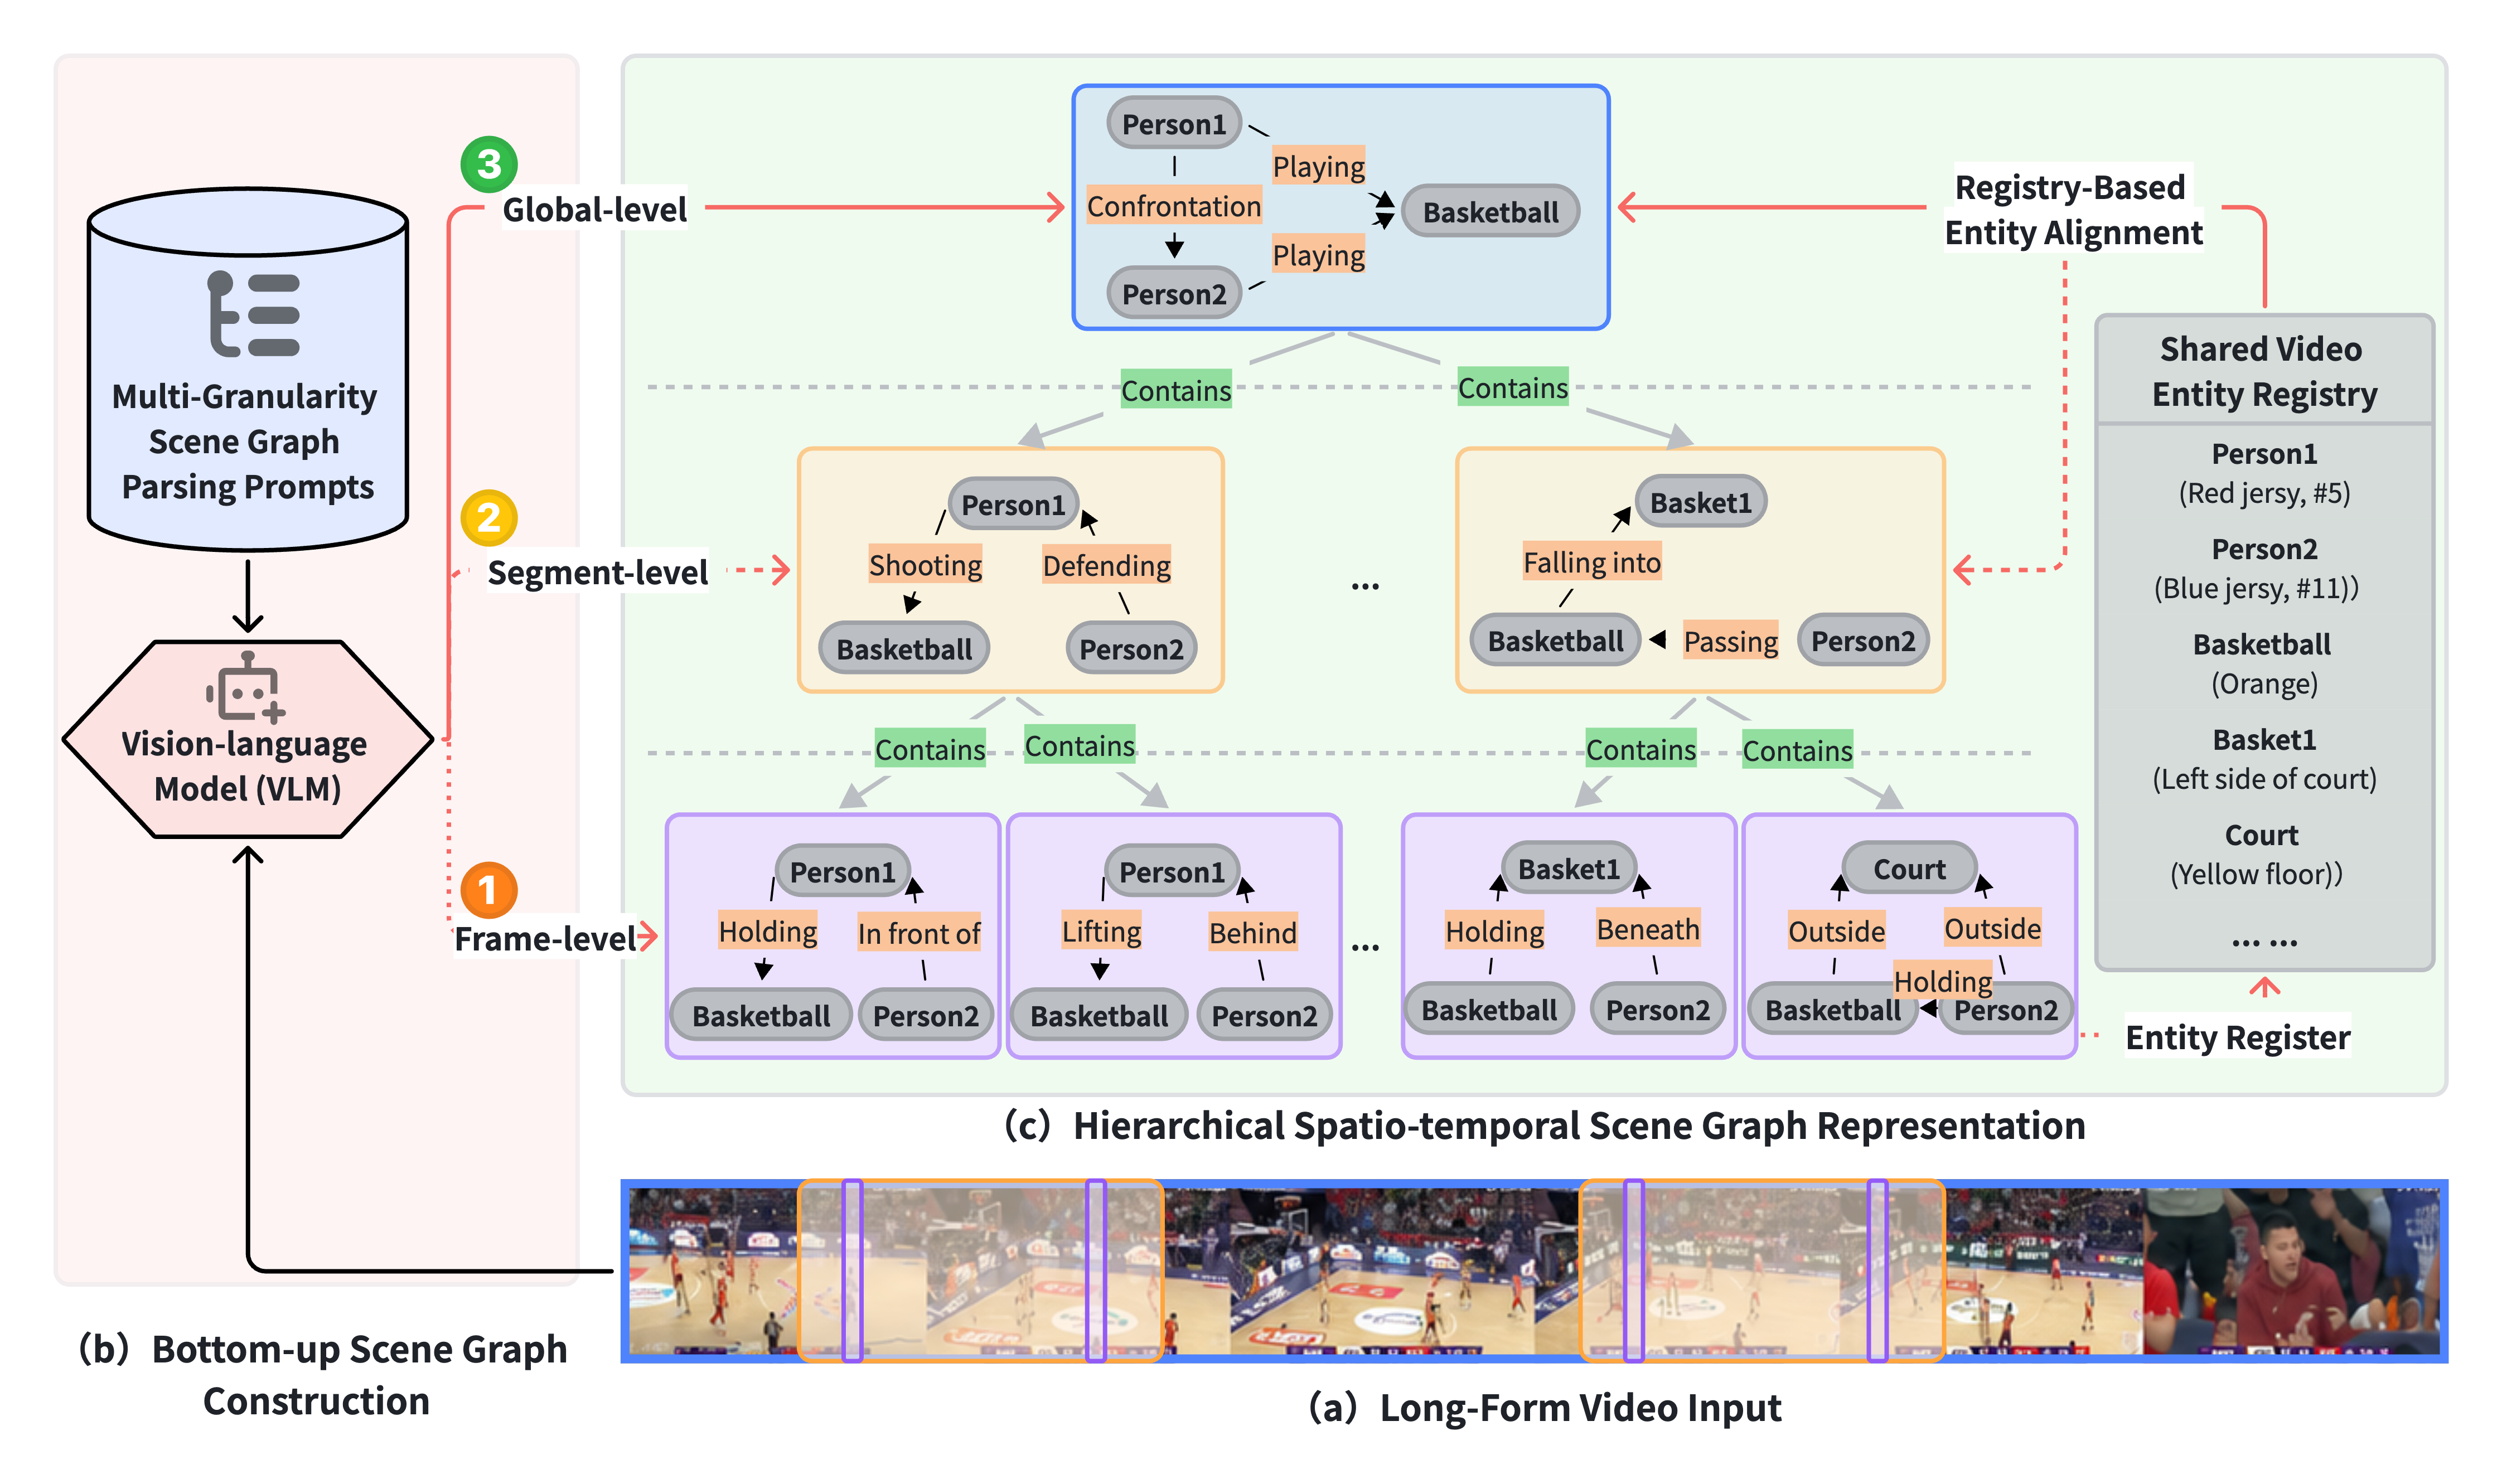
\includegraphics[width=0.95\textwidth]{figures/Graph.png}

  \caption{Overview of the hierarchical spatio-temporal scene graph representation and its bottom-up construction.
  Panel (a) shows the long video input, panel (b) the construction pipeline, and panel (c) the frame-level and segment-level graphs and the global event graph linked by temporal containment, with cross-level entities aligned through a shared registry.}
  \label{fig:graph}

\end{figure*}

\textbf{Agentic video reasoning.}
Directly feeding frame or clip tokens to language models~\cite{video-llava2024,videochat2025} is constrained by context length and computation on hour-scale videos.
LLoVi, Video-of-Thought, VideoRAG, VideoTree, and DrVideo use clip descriptions, stepwise reasoning, retrieval indexes, adaptive trees, and document memory, respectively~\cite{zhang2024simplellm,fei2024videoofthought,videorag2025,videotree2025,drvideo2025}.
OmAgent and MR.~Video decompose long-video processing into smaller tasks~\cite{omagent2024,mrvideo}.
VideoAgent and VideoSeek provide iterative frame retrieval and tool-guided seeking~\cite{videoagent,videoseek}, while VideoMind separates localization, verification, and answering, and VCA uses curiosity-driven tree exploration~\cite{videomind,yang2025vca}.
Vgent links clip nodes through shared entities in a staged retrieval and reasoning pipeline~\cite{vagent2025}.
DVD~\cite{deepvideo2025} organizes global subjects, clip captions, and indexed frames with adaptive multi-granularity tools.
HAVEN~\cite{yin2026haven} couples audiovisual entity cohesion with hierarchical search, and WorldMM~\cite{yeo2026worldmm} retrieves from complementary memories at multiple temporal scales.
SGDAgent's distinctive design couples temporally grounded relation records and cross-level support links with corresponding $GR/SR/FR$ operations.

\section{Methodology}
\label{sec:method}


SGDAgent couples a offline video index with adaptive online retrieval and visual verification.

\subsection{Hierarchical Scene Graph Representation}
\label{sec:representation}

SGDAgent represents a video $V$ with a caption index and a three-level tree-like spatio-temporal scene-graph hierarchy (Figure~\ref{fig:graph}(c)):
\begin{equation}
  \mathcal{I}(V) = \bigl\{C(V),\; E^{\mathrm{video}},\; G^{f},\; G^{s},\; G^{g}\bigr\},
\end{equation}
$C(V)$ is the caption index, while $G^{f}=\{G_i^{f}\}_{i=1}^{N}$, $G^{s}=\{G_j^{s}\}_{j=1}^{M}$, and $G^{g}=(E^{g},\,R^{g})$ denote the frame-level graph sequence, segment-level graph sequence, and global event graph, respectively.
The graph collections include temporal \texttt{contains} and support links to their finer-level evidence.
The shared registry $E^{\mathrm{video}}$ stores entity IDs, names, types, attributes, descriptions, and temporal spans.
The three levels separate instantaneous relations, local interactions, and video-wide events, providing a fixed retrieval interface rather than assuming that every event has the same duration.

\textbf{Frame-level graph.}
Each frame-level graph captures an entity-relation snapshot at a single keyframe:
\begin{equation}
  G_i^{f} = (E_i^{f},\; R_i^{f},\; t_i),
\end{equation}
$E_i^{f} \subseteq E^{\mathrm{video}}$ contains visible entities, while $R_i^{f}$ contains triples $(s,p,o)$ describing spatial relations and instantaneous states, with $s,o \in E_i^{f}$.
$t_i$ is the timestamp.

\textbf{Segment-level graph.}
Each segment-level graph aggregates entity interactions over a short temporal window:
\begin{equation}
  G_j^{s} = (E_j^{s},\; R_j^{s},\;
  [t_j^{\mathrm{s}}, t_j^{\mathrm{e}}],\; F_j),
\end{equation}
$E_j^{s} \subseteq E^{\mathrm{video}}$ contains active entities, while $R_j^{s}$ captures short-term actions, interactions, and temporal relations.
$[t_j^{\mathrm{s}},t_j^{\mathrm{e}}]$ is the segment interval, and $F_j$ contains supporting frame-level graph IDs.
Each relation $(s,p,o,t_{\mathrm{start}},t_{\mathrm{end}},\mathcal{F})$ is grounded by its temporal extent and supporting frames.

\textbf{Global event graph.}
The global event graph abstracts video-wide high-order semantics:
\begin{equation}
  G^{g}=(E^{g},\,R^{g}), \qquad E^{g}\subseteq E^{\mathrm{video}}.
\end{equation}
$E^{g}$ contains entities participating in global events.
$R^{g}$ contains high-order event, state-evolution, temporal, and causal predicates over these entities, grounded in one or more time-bounded intervals.
Cross-level \texttt{contains} links connect the global event graph to its supporting segment graphs.


\begin{figure*}[!tb]
  \centering
  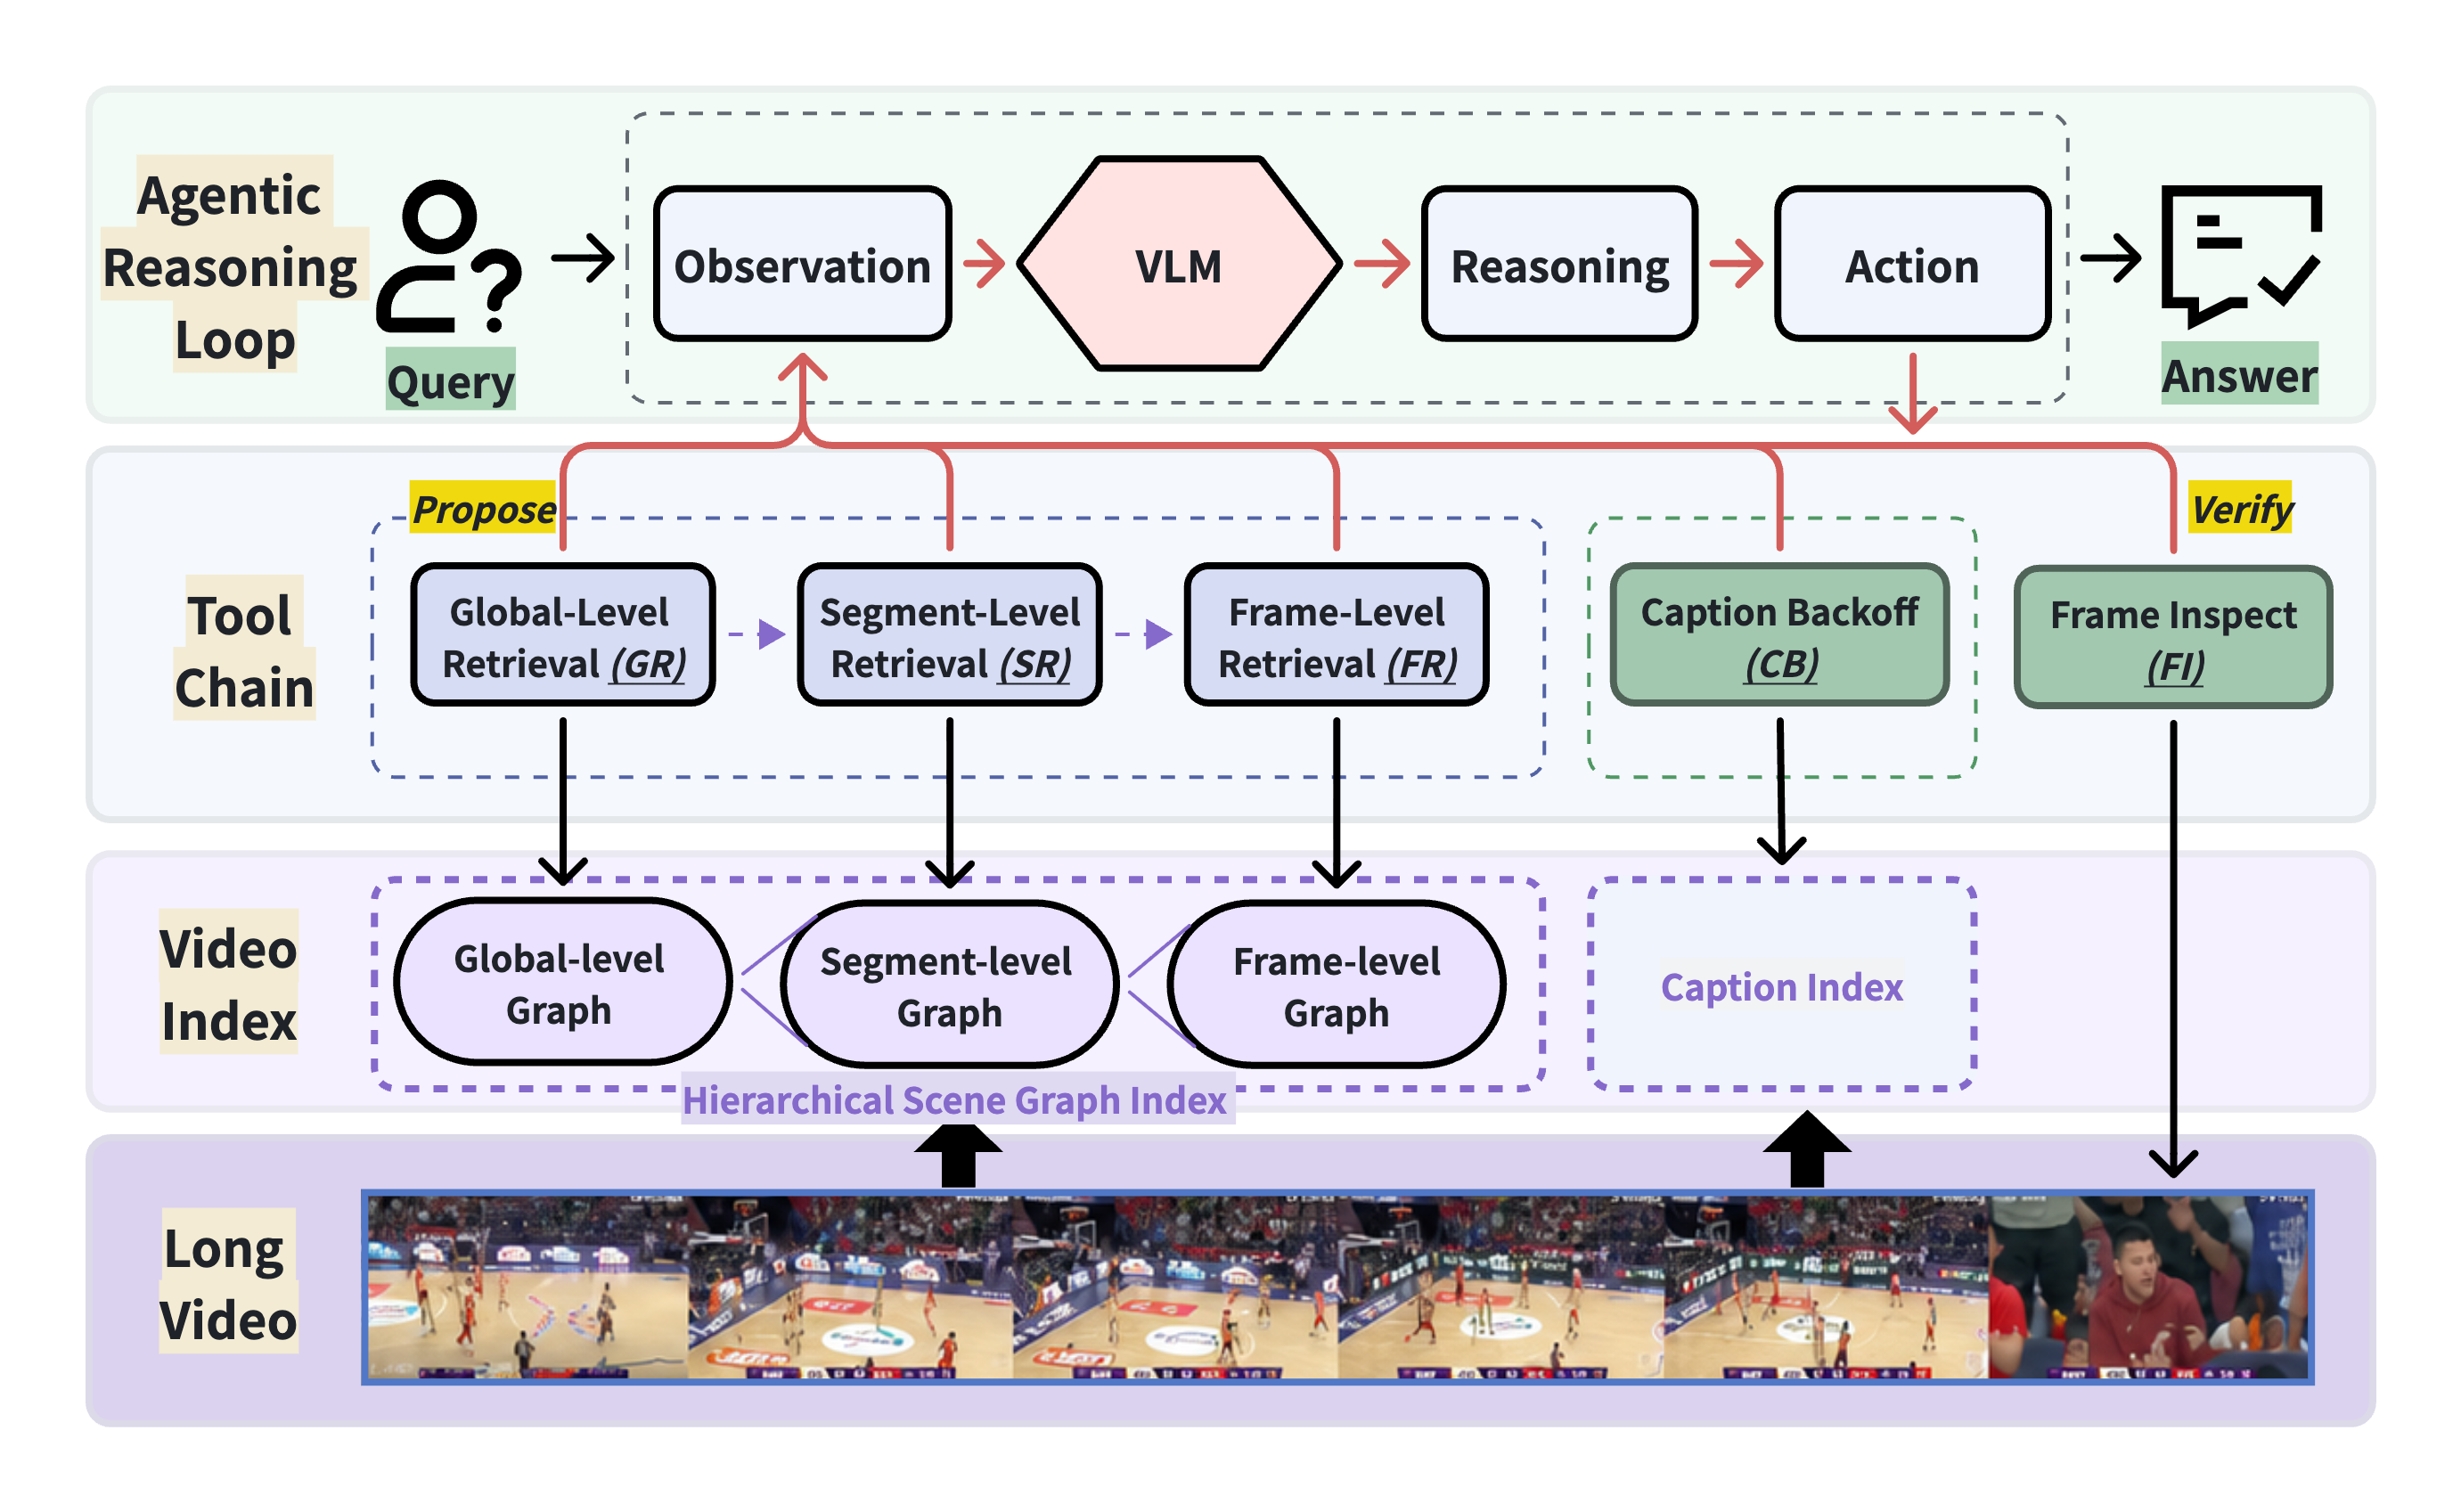
\includegraphics[width=0.95\textwidth]{figures/workflow.png}
  % \vspace{-0.1in}
  \caption{SGDAgent reasoning framework.
  Within the observe-reason-act loop, the agent adaptively selects graph retrieval at global, segment, or frame granularity, caption backoff, or frame inspection over the video index and raw frames.}
  \label{fig:mechanism}
  % \vspace{-0.1in}
\end{figure*}

\subsection{Bottom-up Scene Graph Construction}
\label{sec:construction}

The bottom-up pipeline extracts frame-level graphs, merges them into segment-level graphs, and abstracts frame states and segment actions into global event and causal relations (Figure~\ref{fig:graph}(b)).

\textbf{Frame-level graph extraction and entity registration.}
A vision-language model (VLM) incrementally parses uniformly sampled keyframes, using preceding frame graphs and $E^{\mathrm{video}}$ as context.
The prompt guides it to extract entities, attributes, and relations before greedy identity alignment based on name, description, and type similarity.
Matched records are merged and unmatched entities are registered.
The shared registry links repeated observations of each entity while individual frame graphs retain timestamped attributes and relations.
When parsing returns empty results, neighboring captions from $C(V)$ are used only as auxiliary retry context.

\textbf{Segment-level graph merging.}
Within overlapping windows, the VLM analyzes each clip and its frame graphs to extract entity trajectories, actions, and temporal relations.
Evidence from overlapping regions is used to merge or link actions continuing across adjacent segments.

\textbf{Global event graph construction.}
Temporally adjacent and semantically overlapping segments are grouped into candidate event regions.
A global-level prompt abstracts textual frame and segment records into event, state-evolution, temporal, and causal relations with participating entities and supporting subgraphs; it does not add a new pass over raw pixels.

\textbf{Quality control.}
Schema validation and confidence filtering remove malformed or weak records. Support links retain provenance for subsequent visual checking; generated relations remain retrieval hypotheses rather than verified observations.


\subsection{Scene Graph-Driven Agent}
\label{sec:agent}

\subsubsection{Adaptive agentic reasoning loop.}
Figure~\ref{fig:mechanism} and Algorithm~\ref{alg:search} summarize the agent's observe-reason-act loop~\cite{react2022} over the prebuilt video index.
At step~$t$, state~$H$ contains the question, retrieved candidates, accumulated evidence, and controller signals.
Query-type routing selects the initial tool, after which the LLM selects actions $a_t \in \mathcal{T}$ from the evolving state, and the selected tool updates~$H$.
Confidence gating accepts a proposed answer when its support is sufficient and prioritizes $FI$ when visual confirmation is needed.
If the step budget~$B$ is exhausted, terminal readout returns the best-supported option from the trajectory.

\subsubsection{Tool chain.}
The agent acts over the tool chain $\mathcal{T}=\{GR,\,\allowbreak SR,\,\allowbreak FR,\,\allowbreak FI,\,\allowbreak CB,\,\allowbreak \mathrm{Answer}\}$.
$GR$, $SR$, and $FR$ query the global event graph, segment-level graphs, and frame-level graphs to propose candidates at progressively finer granularity.
The frame-inspection tool $FI$ verifies candidates against raw frames, while caption backoff $CB$ provides a complementary text channel.
Each graph query returns ranked regions, evidence links, and controller signals for confidence-aware descent and verification.

The tool interfaces are
\[
\begin{aligned}
\mathrm{GraphRetrieve}_{\ell}&:(q,\mathrm{scope},k)\\
  &\mapsto(\mathrm{regions}_{1:k},\mathrm{signals}),\\
\mathrm{FrameInspect}&:(\mathrm{window},q)\mapsto\mathrm{evidence},\\
\mathrm{CaptionBackoff}&:(q)\mapsto\mathrm{summary}.
\end{aligned}
\]

All three graph retrievers share a common scorer that ranks a candidate region $w$ against the query $q$ by
\begin{equation}
  \begin{split}
  S(w \mid q) &= S_{\mathrm{lex}}(w,q) \;+\; S_{\mathrm{soft}}(w,q) \\
              &\quad +\; S_{\mathrm{temp}}(w,q).
  \end{split}
\end{equation}
$S_{\mathrm{lex}}$ counts lexical matches, $S_{\mathrm{soft}}$ supplies semantic or fuzzy matches, and $S_{\mathrm{temp}}$ encodes temporal cues.
These are level-specific ranking features, summed with unit outer weights, not calibrated probabilities or equal-magnitude contributions.
Appendix~\ref{sec:retrieval-details} specifies their implementation.
A supplied \texttt{scope} filters candidate intervals before ranking; returned support links identify finer evidence.
Thus routing selects an entry level, while temporal scope and provenance connect successive searches.

\emph{Hierarchical graph retrieval channels.}
Frame-level graph retrieval ($FR$) searches timestamped entity--attribute--relation snapshots for object-level evidence, such as identity, attributes, and spatial relations.
It can operate within a selected segment scope, and its returned timestamps can bound $FI$ to short windows for visual confirmation.
Segment-level graph retrieval ($SR$) searches local interactions globally or within a selected $GR$ interval.
It returns ranked windows, temporal triples, supporting frame links, and controller signals.
These windows can feed $FI$ directly or constrain $FR$ when finer object or relation evidence is needed.
The signals flag weak matches, broad windows, and details requiring visual confirmation.
Global event graph retrieval ($GR$) searches video-wide event, state-evolution, temporal, and causal relations.
It returns ranked intervals with participating entities and supporting segment links, giving causal or plot-level questions an entry point into local evidence.
A selected interval can scope the subsequent $SR$ call to a smaller temporal range.
Retrieval can start at any level, so the hierarchy supports coarse-to-fine search without imposing a fixed traversal on every question.

\emph{Frame inspection and caption backoff.}
$FI$ inspects raw pixels within a candidate window and returns question-conditioned evidence for the final answer.
$CB$ queries the embedding-based caption index when graph vocabulary or coverage is insufficient.
Caption backoff provides another route to candidate discovery, while frame inspection checks the visual details needed to resolve competing answer options.

\begin{algorithm}[!tb]
  \caption{SGDAgent reasoning loop with control strategies: query-type routing (R), confidence gating (CG), and terminal convergence (T).}
  \label{alg:search}
  \begin{algorithmic}[1]
  \footnotesize
  \REQUIRE Video index $\mathcal{I}(V)=\{C(V),E^{\mathrm{video}},G^f,G^s,G^g\}$, query $q$, step budget $B$
  \ENSURE Answer $\hat{a}$
  \STATE $H \leftarrow \mathrm{InitState}(q)$
  \FOR{$t=1,\ldots,B$}
      \STATE $a_t \leftarrow \mathrm{QueryTypeRoute}(\mathrm{LLM}(H),q,t)$
        \hfill \textcolor{blue!60!black}{\small\textbf{[R]}}
      \IF{$a_t \in \{GR,SR,FR\}$}
          \STATE $H \leftarrow \mathrm{GraphRetrieve}(H,a_t,q,\mathcal{I}(V))$
          \IF{$\mathrm{WeakGraphSignal}(H)$}
              \STATE $H \leftarrow \mathrm{CaptionBackoff}(H,q,C(V))$
                \hfill \textcolor{blue!60!black}{\small\textbf{[CG]}}
          \ENDIF
      \ELSIF{$a_t=CB$}
          \STATE $H \leftarrow \mathrm{CaptionBackoff}(H,q,C(V))$
      \ELSIF{$a_t=FI$}
          \STATE $H \leftarrow \mathrm{FrameInspect}(H,q)$
      \ELSIF{$a_t=\mathrm{Answer} \land \mathrm{ConfidenceGate}(H)$}
          \RETURN $\mathrm{Readout}(H)$
            \hfill \textcolor{blue!60!black}{\small\textbf{[CG]}}
      \ELSIF{$a_t=\mathrm{Answer}$}
          \STATE $H \leftarrow \mathrm{AppendGateFeedback}(H)$
      \ENDIF
  \ENDFOR
  \RETURN $\mathrm{TerminalReadout}(H)$
    \hfill \textcolor{blue!60!black}{\small\textbf{[T]}}
  \end{algorithmic}
\end{algorithm}


\subsubsection{Agent control strategies.}
In the implementation, query-type routing (R) uses ordered question-text rules for the first tool: visual-detail cues select $FI$, causal or plot cues select $GR$, temporal-localization cues select $SR$, and object-relation cues select $FR$; the default is $GR$.
For $t>1$, \texttt{QueryTypeRoute} passes through the LLM's action, selected from observations and controller guidance.
Confidence gating (CG) blocks answers based only on weak or localization-only evidence and appends feedback to $H$ for another retrieval or inspection step.
Controller signals describe match quality, region granularity, and the need for visual confirmation, distinguishing candidate localization from answer evidence.
Terminal convergence (T) reads out the best-supported option when the budget is exhausted.
Appendix~\ref{sec:routing-details} gives the rule boundaries and optional context inputs.

\begin{table*}[!tb]
  \centering
  \small
  \setlength{\tabcolsep}{2.5pt}
  \begin{tabularx}{\textwidth}{@{}lXcccc@{}}
    \toprule
    & & \textbf{LVBench} & \textbf{LongVideoBench} & \textbf{Video-MME} & \textbf{EgoSchema} \\
    \textbf{Method} & \textbf{Model setup}
    & \textit{full}
    & \textit{Val, overall}
    & \textit{Long, w/o sub}
    & \textit{Val 500} \\
    \midrule
    \multicolumn{6}{l}{\textit{Commercial VLMs}} \\
    Gemini-1.5-Pro~\cite{gemini15}
      & -             & 33.1 & 64.0 & 67.4 & -   \\
    Gemini-2.0-Flash~\cite{gemini15}
      & -             & 48.3 & - & 63.0 & 71.2   \\
    GPT-4o~\cite{gpt4o}
      & -             & 48.9 & 66.7 & 65.3 & 70.4 \\
    OpenAI o3~\cite{o3}
      & -             & 57.1 & 67.5 & 64.7 & 63.2 \\
    Gemini-2.5-Pro~\cite{gemini25}
      & -             & 67.4 & -   & -   & -   \\
    Seed1.5-VL-Thinking~\cite{seed}
      & -             & 64.6 & - & -   & -   \\
    \midrule
    \multicolumn{6}{l}{\textit{Open-Source VLMs}} \\
    % mPLUG-Owl3~\cite{} & 78B           & 43.5 & 59.8 & 50.1  & -   \\
    InternVL2.5-78B~\cite{internvl}
      & -             & 43.6 & 63.6 & 62.6  & -   \\
    % AdaRETAKE~\cite{} & 72B           & 53.3 & 67.0 & 65.0 & -   \\
    Qwen2.5-VL-72B~\cite{qwen}
      & -             & 47.7 & 60.7 & 63.9 & -   \\
    \midrule
    \multicolumn{6}{l}{\textit{Video Agents}} \\
    VideoAgent~\cite{videoagent}
      & -            & 29.3 & -   & -   & 63.2 \\
    VideoMind~\cite{videomind}
      & 7B model      & 40.8 & -   & -   & -   \\
    MR.~Video~\cite{mrvideo}
      & Gemini Flash  & 60.8 & -   & 61.8 & 73.0 \\
    VideoSeek~\cite{videoseek}
      & GPT-5         & 68.4 & -   & -   & -   \\
    DVD~\cite{deepvideo2025}
      & o4-mini (reasoning) / o3 (FI)        & 70.2 & -   & -   & -   \\
    DVD~\cite{deepvideo2025}
      & o3            & 74.2 & 71.6 & 67.3 & 76.6 \\
    \midrule
    \multicolumn{6}{l}{\textit{Ours}} \\
    SGDAgent
      & o4-mini (reasoning) / o3 (FI)      & 73.0 & 71.2 & 65.1 & 74.0 \\
    SGDAgent
      & o3            & \textbf{75.9} & \textbf{74.0} & \textbf{69.0} & \textbf{77.4} \\
    \bottomrule
  \end{tabularx}
  \caption{Accuracy comparison on four long-video understanding benchmarks.
  Methods are grouped by family, and results serve as reference comparisons because model setups and evaluation settings differ. (FI: frame inspection.)}
  \label{tab:main_comparison}

\end{table*}


% -----------
%  Experiment 1: Video-index Composition and Scene-graph Hierarchy
% -----------

\begin{table*}[!tb]
  \centering
  \small
  \setlength{\tabcolsep}{1.45pt}
  \renewcommand{\arraystretch}{1.10}
  \begin{tabular}{@{}lc ccc@{\hspace{6pt}}ccc@{\hspace{6pt}}cccccc@{}}
    \toprule
    \multirow{2}{*}{\textbf{Configuration}} &
    \multirow{2}{*}{\shortstack{\textbf{Caption}\\\textbf{(C)}}} &
    \multicolumn{3}{c}{\shortstack{\textbf{Scene-graph}\\\textbf{hierarchy}}} &
    \multicolumn{3}{c}{\shortstack{\textbf{Agent control}\\\textbf{strategies}}} &
    \multicolumn{6}{c}{\shortstack{\textbf{Metrics}\\\strut}} \\
    \cmidrule(lr){3-5}\cmidrule(lr){6-8}\cmidrule(l){9-14}
    & &
    \makebox[0.18in][c]{\textbf{F}} &
    \makebox[0.18in][c]{\textbf{S}} &
    \makebox[0.18in][c]{\textbf{G}} &
    \makebox[0.18in][c]{\textbf{R}} &
    \makebox[0.18in][c]{\textbf{CG}} &
    \makebox[0.18in][c]{\textbf{T}} &
    \makebox[0.56in][c]{\shortstack{\textbf{End-to-end}\\\textbf{acc.}\textsuperscript{($\uparrow$)}}} &
    \makebox[0.56in][c]{\shortstack{\textbf{Answered}\\\textbf{acc.}\textsuperscript{($\uparrow$)}}} &
    \makebox[0.56in][c]{\shortstack{\textbf{Answer}\\\textbf{rate}\textsuperscript{($\uparrow$)}}} &
    \makebox[0.56in][c]{\shortstack{\textbf{FTT}\\\textbf{rate}\textsuperscript{($\downarrow$)}}} &
    \makebox[0.56in][c]{\shortstack{\textbf{Avg. LLM}\\\textbf{calls}\textsuperscript{($\downarrow$)}}} &
    \makebox[0.56in][c]{\shortstack{\textbf{Avg. FI}\\\textbf{calls}\textsuperscript{($\downarrow$)}}} \\
    \midrule
    \emph{Base}       & $\checkmark$ &              &              &              &              &              &              & 54.8 & 65.7 & 83.5 & 16.5 & 3.7  & 1.1 \\
    \emph{Base}\textsuperscript{C+F}  & $\checkmark$ & $\checkmark$ &              &              &              &              &              & 59.2 & 69.0 & 85.8 & 14.2 & 4.9  & 2.4 \\
    \emph{Base}\textsuperscript{C+F+S} & $\checkmark$ & $\checkmark$ & $\checkmark$ &              &              &              &              & 62.8 & 72.0 & 87.2 & 12.8 & 9.6  & 5.1 \\
    \emph{Base}\textsuperscript{F+S+G} &              & $\checkmark$ & $\checkmark$ & $\checkmark$ &              &              &              & 58.0 & 69.1 & 83.9 & 16.1 & 4.4 & 1.6 \\
    \emph{SGDAgent}\textsuperscript{0} & $\checkmark$ & $\checkmark$ & $\checkmark$ & $\checkmark$ &              &              &              & 64.4 & 72.2 & 89.2 & 10.8 & \textbf{2.9}  & 1.4 \\
    \midrule
    \emph{SGDAgent}\textsuperscript{R} & $\checkmark$ & $\checkmark$ & $\checkmark$ & $\checkmark$ & $\checkmark$ &              &              & 69.5 & \textbf{75.1} & 92.6 & 7.4 & 3.0 & 1.3 \\
    \emph{SGDAgent}\textsuperscript{R+CG} & $\checkmark$ & $\checkmark$ & $\checkmark$ & $\checkmark$ & $\checkmark$ & $\checkmark$ &              & 70.7 & 74.6 & 94.8 & 5.2 & 3.5 & 1.4 \\
    \emph{SGDAgent}\textsuperscript{R+T} & $\checkmark$ & $\checkmark$ & $\checkmark$ & $\checkmark$ & $\checkmark$ &              & $\checkmark$ & 70.8 & 74.1 & 95.6 & 4.4 & 3.1 & 1.2 \\
    \midrule
    \emph{SGDAgent} & $\checkmark$ & $\checkmark$ & $\checkmark$ & $\checkmark$ & $\checkmark$ & $\checkmark$ & $\checkmark$ & \textbf{73.0} & 74.2 & \textbf{98.4} & \textbf{1.6}  & 3.4  & \textbf{1.0} \\
    \bottomrule
  \end{tabular}
  \caption{Matched-setting LVBench ablations of video-index composition, scene-graph hierarchy, and agent control.
  C denotes the caption index; F and S denote frame-level and segment-level graphs, and G denotes the global event graph; R, CG, and T denote query-type routing, confidence gating, and terminal convergence.
  FTT denotes the failed-to-terminate rate; accuracy and rates are percentages, while large language model (LLM) and frame-inspection (FI) calls are per-question averages.}
  \label{tab:component_ablation}

\end{table*}



\begin{figure*}[!tb]
  \centering
   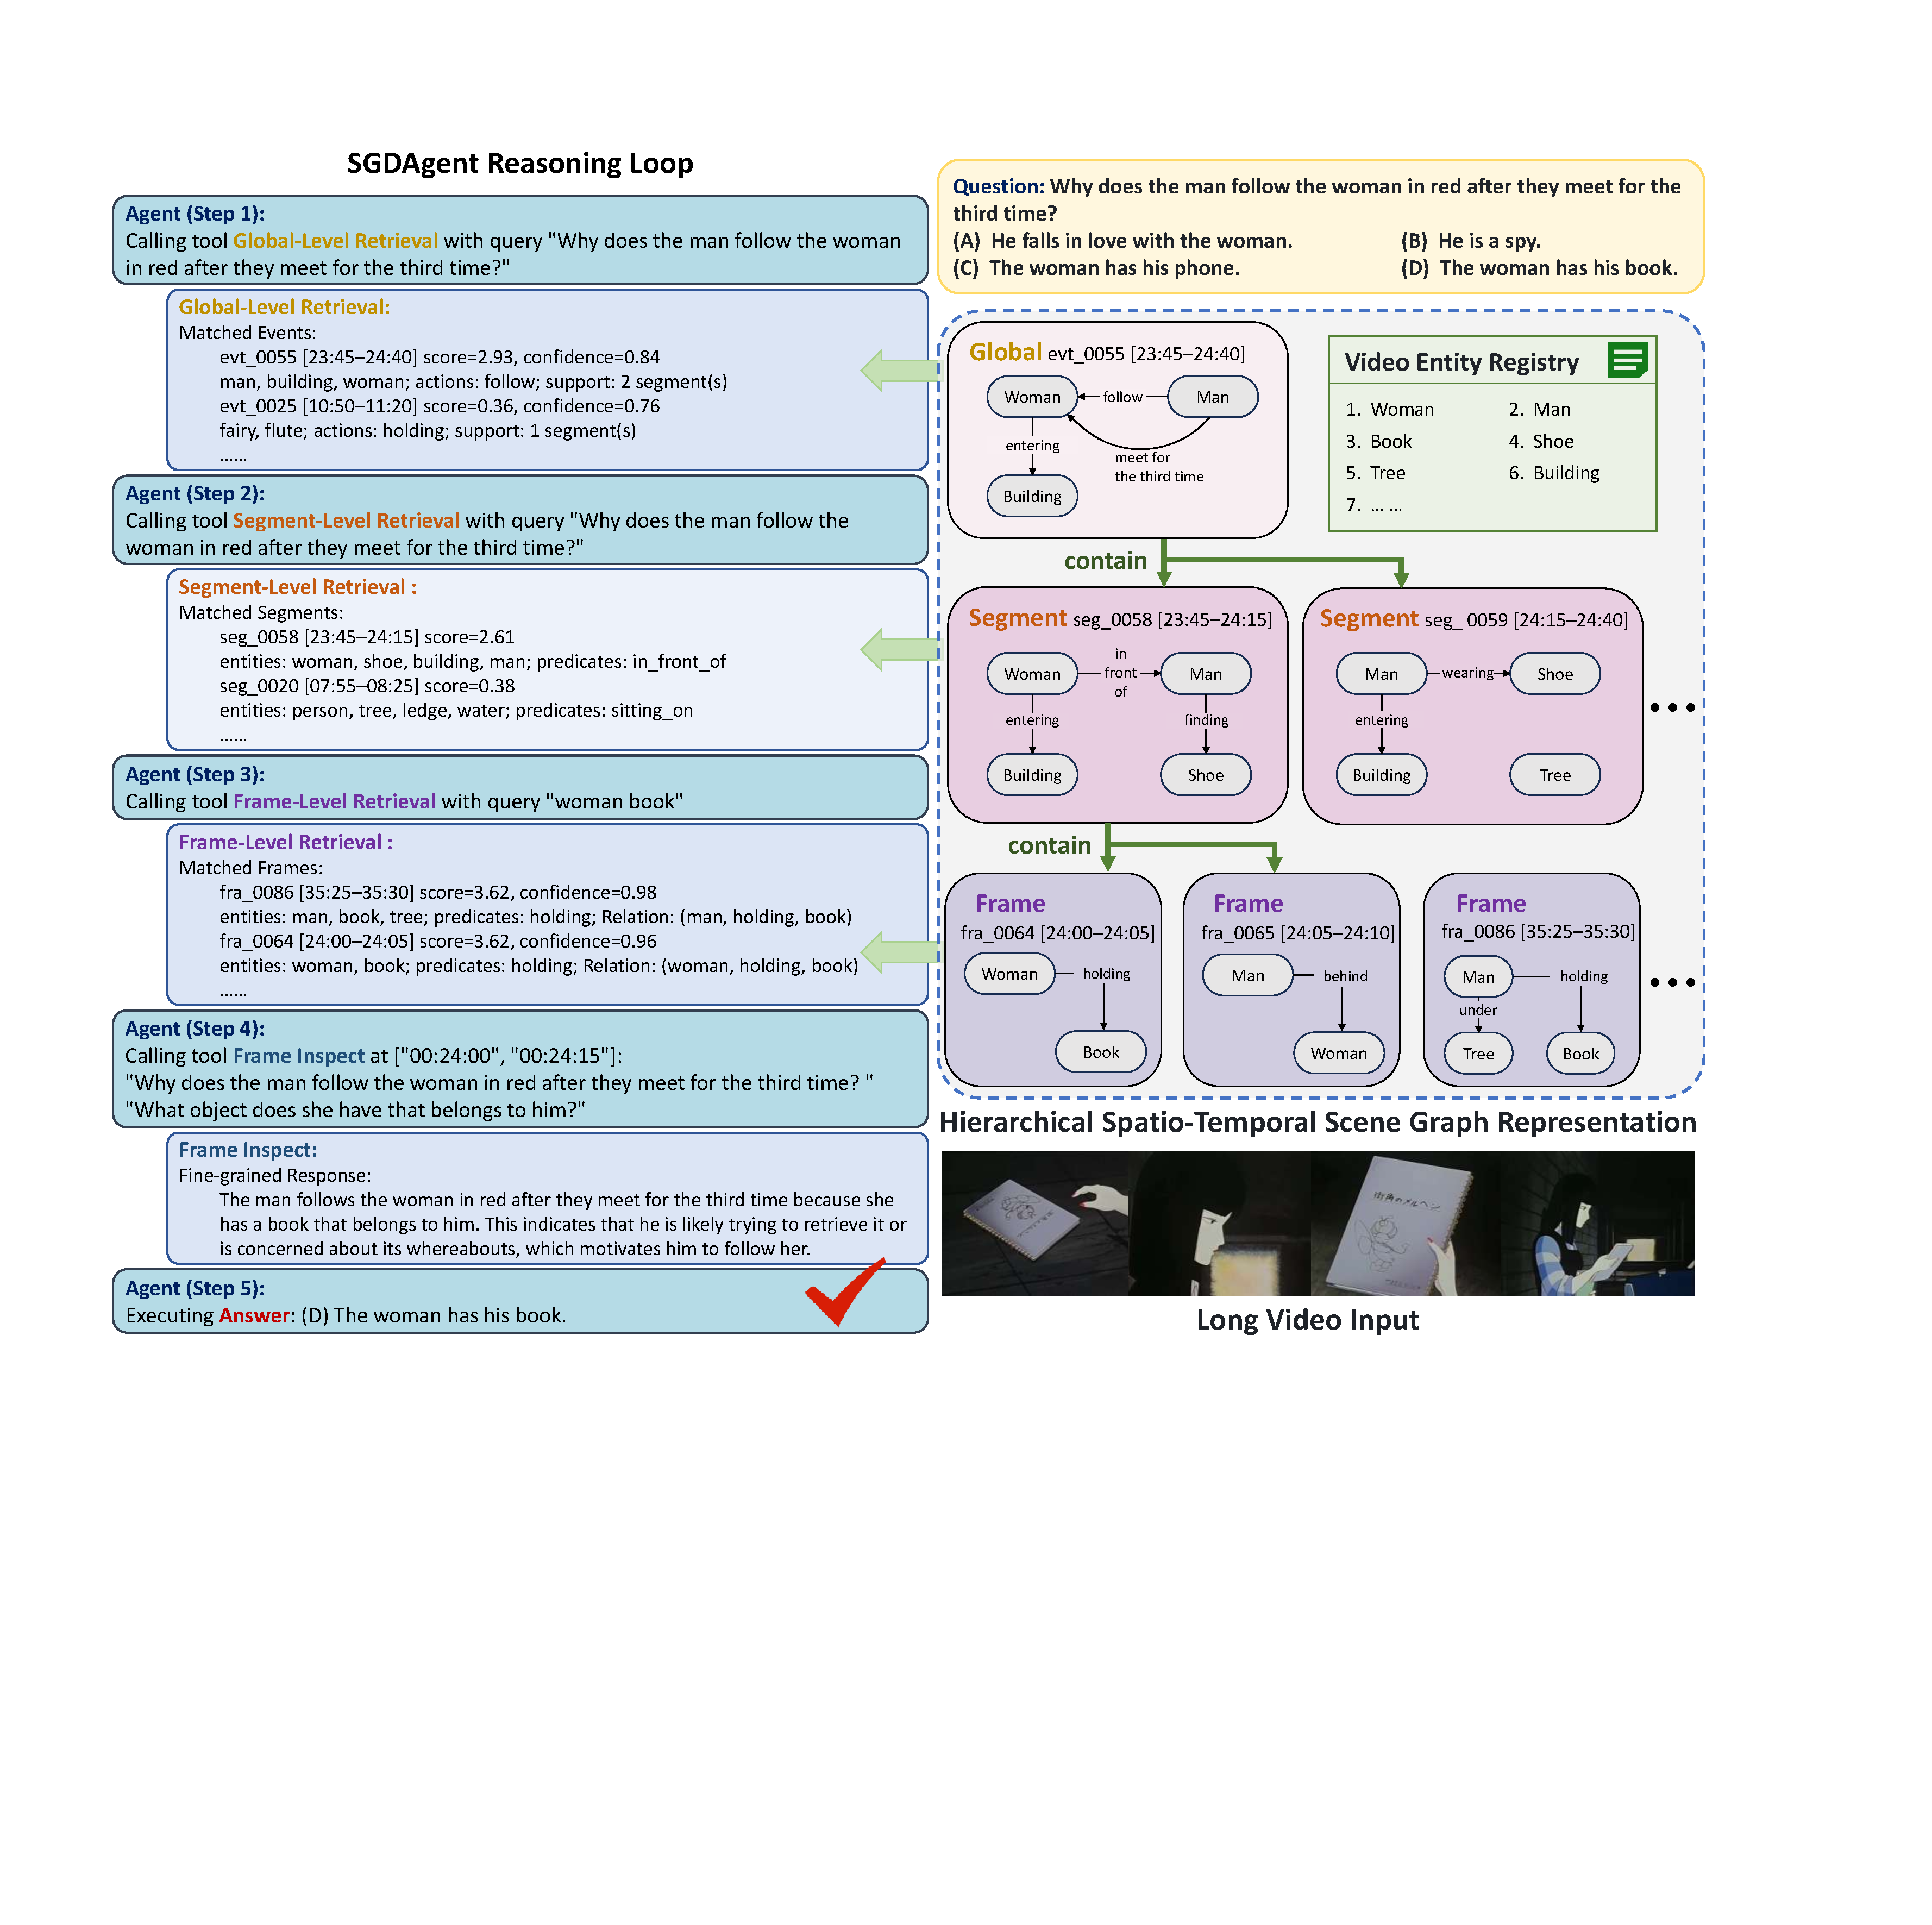
\includegraphics[width=\textwidth]{figures/Case.pdf}
  %  \vspace{-0.1in}
  \caption{An LVBench case~\cite{lvbench} illustrates how SGDAgent escapes the frame-inspect trap~\cite{deepvideo2025} (qid: \texttt{q01CUy\_gwdU\_\_121}).
  The trajectory shows coarse-to-fine localization followed by frame inspection.}
  \label{fig:trajectory}

\end{figure*}


\section{Experiments}
\label{sec:experiments}

% ============================================================
%  Section 4.1  --  Experimental Setup
% ============================================================

\subsection{Experimental Setup}
\label{sec:setup}

\textbf{Datasets.}
We evaluate SGDAgent on the full LVBench split~\cite{lvbench}, LongVideoBench validation~\cite{longvideobench2024}, Video-MME Long without subtitles~\cite{videomme2024}, and EgoSchema Val 500~\cite{egoschema2023}.
All SGDAgent results in Table~\ref{tab:main_comparison} are our runs on these splits.
LVBench, which contains 1{,}549 questions over 103 long videos, is additionally used for matched-setting ablations and a qualitative illustration.

% ============================================================
%  Main Comparison Table -- spans 4 benchmarks
% ============================================================


\textbf{Implementation details.}
By default, we use \texttt{o4-mini} as the reasoning model and \texttt{gpt-4.1} for frame-level graph extraction.
Entity alignment weights name, description, and type similarity by 0.7, 0.2, and 0.1, respectively, with a merge threshold of 0.78.
Segment-level graphs are constructed using 30-second sliding windows with 5-second overlap.
Before global abstraction, segments are grouped into candidate event regions using a maximum temporal gap of 12~seconds, relation- and predicate-overlap thresholds of 0.18 and 0.22, and shared entities as an additional merge cue.
Frame inspection uses at most 50~frames per call, while $GR$, $SR$, and $FR$ return up to 5, 6, and 8 candidates, respectively.
Building the LVBench scene graph index takes about 7.94 hours with four workers, including about 121 seconds for global event graph construction.
The video index is constructed once and reused across all questions.
For the caption index, we follow the construction and embedding-based retrieval protocol of DVD~\cite{deepvideo2025} for a fair comparison.
Matched LVBench configurations share the reasoning model, frame-inspection VLM, captions, answer choices, and budgets, varying only index composition, scene-graph hierarchy, and agent control.

\textbf{Evaluation metrics.}
End-to-end accuracy divides correct answers by all questions; answered accuracy divides by answered questions.
Answer rate is the fraction answered and equals $1-\mathrm{FTT}$, where FTT includes empty outputs, runtime failures, and non-convergent trajectories.
LVBench ablation percentages are independently computed and rounded to one decimal place.
Following caption-index agents~\cite{videoagent,deepvideo2025,drvideo2025}, we assess index utility through downstream QA and component ablations; direct graph evaluation is discussed in Limitations.

\subsection{Main Results}
\label{sec:results}

Table~\ref{tab:main_comparison} reports SGDAgent and published baselines across four benchmarks.
With \texttt{o4-mini}, SGDAgent achieves 73.0\% on LVBench and 71.2\% on LongVideoBench, approaching DVD's reported \texttt{o3} results of 74.2\% and 71.6\%.
The \texttt{o3} configuration improves all four SGDAgent scores, reaching 75.9\% on LVBench, 74.0\% on LongVideoBench, 69.0\% on Video-MME Long, and 77.4\% on EgoSchema.
The corresponding reported DVD results are 74.2\%, 71.6\%, 67.3\%, and 76.6\%.
The consistent improvements within SGDAgent indicate that its structured retrieval interface can also benefit from a stronger reasoning model.
These comparisons provide context for the system's performance; settings differ across methods, so the matched LVBench experiments carry the component-level analysis.

\subsection{Ablation Study}

Table~\ref{tab:component_ablation} compares index composition and agent control under matched LVBench settings.
\emph{Base} denotes the caption-only baseline, and \emph{SGDAgent}$^0$ the complete index without controls.
Superscripts list index components for \emph{Base} and controls for \emph{SGDAgent}.

\textbf{Index composition.}
Graph-only \emph{Base}$^{F+S+G}$ reaches 58.0\%, compared with 54.8\% for caption-only \emph{Base}, while their combination reaches 64.4\%.
Adding frame and segment channels progressively improves end-to-end accuracy to 59.2\% and 62.8\%.
Adding the global graph raises it to 64.4\% and reduces LLM calls from 9.6 to 2.9 and frame inspections from 5.1 to 1.4.
These results support complementary caption and graph channels and more economical search with the global level.
Captions retain broad lexical coverage, while frame and segment graphs expose entity relations and local interactions for candidate discovery.
The global level then supplies longer-range event context to guide this local search.
We evaluate the coupled index and retrieval design, rather than isolating containment links from the additional graph-derived information.

\textbf{Agent control.}
Routing raises answered accuracy from 72.2\% to 75.1\% and answer rate from 89.2\% to 92.6\%.
Adding CG or T to routing raises end-to-end accuracy from 69.5\% to 70.7\% or 70.8\%, respectively, mainly by resolving more questions, with a slight decrease in answered accuracy.
All three controls yield 73.0\% end-to-end accuracy, 74.2\% answered accuracy, and 98.4\% answer rate.
Thus the controller improves coverage as well as answer quality; these contrasts measure its effect with the graph index present.
The separate accuracy and coverage measures clarify their roles: routing improves the quality of answered questions, whereas CG and T mainly recover unresolved trajectories through evidence escalation and terminal readout.
The smaller differences are descriptive point estimates, not significance claims.

\textbf{Online efficiency.}
The full system uses 3.4 LLM calls and 1.0 frame inspections per question, compared with 3.7 and 1.1 for \emph{Base}.
The main reduction occurs when the global level is added to frame and segment retrieval.
Frame and segment retrieval require more local exploration, while the global level reduces this cost through broader event context.
These counts measure online search after index construction, not total compute; the offline index is reused across questions.

\subsection{Analysis of Agentic Reasoning Behavior}
\label{sec:analysis}

Figure~\ref{fig:trajectory} schematically illustrates the roles of $GR$, $SR$, $FR$, and $FI$ in a repeated-encounter question: ``Why does the man follow the woman in red after they meet for the third time?''
The correct answer is that the woman has his book.
The question combines event-level localization with object-level evidence, motivating targeted visual verification after graph retrieval.
The caption-only path illustrates repeated frame inspection without a relational anchor, while the graph-guided path proposes an event, identifies candidate interactions and book possession, and checks the raw frames.
The displayed snippets illustrate tool roles rather than a complete execution log of strictly nested scopes.
This illustration complements the quantitative evidence from the matched ablation.

\section{Conclusion}

SGDAgent co-designs a hierarchical scene-graph video index and level-specific retrieval for long-video reasoning.
Shared identities and temporal links connect frame observations, local interactions, and global events to guide visual verification.
Matched LVBench comparisons show complementary graph and caption evidence, reduced online search with the global level, and improved answer coverage through agent control.
The four-benchmark evaluation further demonstrates competitive performance across long-video settings.
This offers a structured interface between video abstraction, candidate retrieval, and visual verification.

\section*{Limitations}
Direct evaluation of scene graph construction quality is challenging because standardized annotations for open-vocabulary relations, cross-frame identity, and hierarchical temporal support are limited, and different graphs may encode equivalent evidence.
Following prior caption-index agents, we emphasize downstream QA.
Future evidence-linked annotations could support graph consistency and error-propagation analyses.
We use fixed temporal windows and retrieval heuristics for reproducibility.
Token budgets and financial constraints led us to prioritize core ablations over extensive sensitivity studies.
Broader sensitivity studies and query-adaptive refinement could clarify robustness and improve the balance between indexing cost and retrieval quality.



%%
%% Bibliography
%%
\bibliography{references}

\clearpage
\appendix
\setcounter{table}{0}
\setcounter{figure}{0}
\setcounter{equation}{0}
\renewcommand{\thetable}{S\arabic{table}}
\renewcommand{\thefigure}{S\arabic{figure}}
\renewcommand{\theequation}{S\arabic{equation}}

\section{Additional Empirical Results}
\label{sec:supp-analysis}

This section provides diagnostic views of the aggregate LVBench results reported in the main paper while retaining the same matched evaluation setting.

\subsection{Category-Level Diagnostic Breakdown}

LVBench assigns one or more capability tags to each question.
The most frequent tags are entity recognition (677 questions, 43.7\%), event understanding (647, 41.8\%), key information retrieval (291, 18.8\%), temporal grounding (220, 14.2\%), reasoning (201, 13.0\%), and summarization (58, 3.7\%).
Table~\ref{tab:supp-category} compares the caption-only baseline and SGDAgent across these categories.
% To align the category-wise diagnostic ratios with the matched setting, the SGDAgent column is uniformly normalized to the 73.0\% overall accuracy reported in the main paper.
We use this breakdown only to compare relative category trends; it does not replace the directly measured overall result or constitute an additional experiment.

\begin{center}
  \centering
  \small
  \setlength{\tabcolsep}{3pt}
  \begin{tabular}{@{}lrrr@{}}
    \toprule
    \textbf{Category} &
    \textbf{$n$} &
    \textbf{Caption-only} &
    \shortstack{\textbf{SGDAgent}\\\textbf{(norm.)}} \\
    \midrule
    Entity Recognition & 677 & 55.2 & 71.3 \\
    Event Understanding & 647 & 54.1 & 71.9 \\
    Key Info. Retrieval & 291 & 65.6 & 83.2 \\
    Temporal Grounding & 220 & 54.1 & 76.3 \\
    Reasoning & 201 & 48.3 & 60.5 \\
    Summarization & 58 & 43.1 & 68.6 \\
    \bottomrule
  \end{tabular}
  \captionof{table}{Category-level diagnostic end-to-end accuracy (\%) on LVBench.  SGDAgent values are uniformly normalized to the main-paper overall result; questions may carry multiple capability tags.}
  \label{tab:supp-category}
\end{center}

The differences are positive across all six categories.
The largest differences appear in summarization ($+25.5$ points) and temporal grounding ($+22.2$), followed by event understanding ($+17.8$), key information retrieval ($+17.6$), entity recognition ($+16.1$), and reasoning ($+12.2$).
This pattern is consistent with the role of hierarchical graph retrieval in narrowing long videos to plausible temporal regions.
The smaller reasoning difference is also consistent with the continued need for fine-grained visual confirmation through $FI$ after localization.

\subsection{Additional Insights from the Matched Ablation}

Table~\ref{tab:supp-deltas} reports paired differences computed directly from the one-decimal values in the main-paper ablation table.
C denotes the caption index; F, S, and G denote the three graph levels; and R, CG, and T denote the three control strategies.

\begin{center}
  \centering
  \small
  \setlength{\tabcolsep}{1.9pt}
  \begin{tabular}{@{}lrrrrr@{}}
    \toprule
    \textbf{Change} &
    \textbf{$\Delta$E2E} &
    \textbf{$\Delta$Ans.} &
    \textbf{$\Delta$Rate} &
    \textbf{$\Delta$LLM} &
    \textbf{$\Delta$FI} \\
    \midrule
    C $\rightarrow$ C+F                 & +4.4 & +3.3 & +2.3 & +1.2 & +1.3 \\
    C+F $\rightarrow$ C+F+S             & +3.6 & +3.0 & +1.4 & +4.7 & +2.7 \\
    C+F+S $\rightarrow$ C+F+S+G          & +1.6 & +0.2 & +2.0 & $-6.7$ & $-3.7$ \\
    \midrule
    No ctl. $\rightarrow$ R              & +5.1 & +2.9 & +3.4 & +0.1 & $-0.1$ \\
    R $\rightarrow$ R+CG                & +1.2 & $-0.5$ & +2.2 & +0.5 & +0.1 \\
    R $\rightarrow$ R+T                 & +1.3 & $-1.0$ & +3.0 & +0.1 & $-0.1$ \\
    R $\rightarrow$ R+CG+T              & +3.5 & $-0.9$ & +5.8 & +0.4 & $-0.3$ \\
    \bottomrule
  \end{tabular}
  \captionof{table}{Paired differences derived from the main-paper component ablation.  Accuracy and answer-rate differences are percentage points; call-count differences are per question.}
  \label{tab:supp-deltas}
\end{center}

The main-paper ablation reveals two complementary effects.
Frame- and segment-level graphs broaden structured candidate discovery but require more local exploration.
The global event graph reverses this cost trend by routing the same local tools to a smaller temporal scope, indicating that its main benefit is search compression rather than direct visual verification.

The control variants show a related accuracy--coverage trade-off.
Confidence gating and terminal convergence recover more unresolved trajectories, while answered accuracy changes only slightly.
The conditional contrasts support a complementary interpretation rather than an additive decomposition: gating escalates uncertain evidence, whereas terminal convergence prevents remaining trajectories from exhausting the step budget.

\section{Additional Reproducibility Details}
\label{sec:supp-reproducibility}

We next document the implementation choices that support reproduction and clarify how the graph hierarchy and online agent are operationalized.

\subsection{Frame-Graph Extraction and Normalization}

The main paper specifies the model roles, graph hierarchy, and matched evaluation protocol.
This subsection supplies the finer-grained frame-level extraction, sampling, and normalization settings.
Table~\ref{tab:supp-settings} summarizes the extraction and sampling configuration.

\begin{center}
  \centering
  \small
  \setlength{\tabcolsep}{4pt}
  \begin{tabularx}{\columnwidth}{@{}lY@{}}
    \toprule
    \textbf{Component} & \textbf{Setting} \\
    \midrule
    Frame-graph extraction &
    \texttt{gpt-4.1}, temperature 0, at most 800 output tokens \\
    Frame sampling &
    candidates sampled every 5 seconds from 2 FPS decoded frames; when more than 120 candidates are available, 120 are uniformly retained over the full video \\
    \bottomrule
  \end{tabularx}
  \captionof{table}{Additional frame-level construction settings.}
  \label{tab:supp-settings}
\end{center}

For each sampled keyframe, the extractor produces a compact set of typed entities and directed relation triples.
The following core instruction specifies the output contract.
It should not be read as the complete model input: the preceding-frame graphs and video-level entity-registry context are provided as described in the main paper.

\begin{lstlisting}
System:
You produce strict JSON only.

User:
Extract a compact frame-level scene graph from this image.
Return strict JSON with schema:
{"entities":[{"local_id":"e1","name":"person","type":"person",
"attributes":["standing"],"desc_text":"short description",
"confidence":0.0}],
"relations":[{"s":"e1","p":"holding","o":"e2","confidence":0.0}]}.
Rules: keep 1-8 salient entities, 0-12 relations, relation predicate in snake_case.
\end{lstlisting}

The raw response is normalized deterministically before registry matching.
Post-processing lower-cases entity names and relation predicates.
Entity types are restricted to \texttt{person}, \texttt{object}, \texttt{scene}, \texttt{animal}, \texttt{vehicle}, \texttt{food}, \texttt{text}, \texttt{location}, \texttt{building}, \texttt{clothing}, \texttt{instrument}, and \texttt{plant}.
Out-of-vocabulary types map to \texttt{object}.
Meta-level terms such as \texttt{video}, \texttt{camera}, \texttt{subtitle}, and \texttt{background} are removed.
Relation predicates outside the spatial, interaction, and state/action whitelist are discarded, and confidence values are clipped to $[0,1]$.
If extraction yields no usable entity, neighboring caption text is used only as auxiliary retry context, consistent with the construction procedure in the main paper.

\subsection{Cross-Frame Entity Alignment}

Normalized frame graphs are processed sequentially into the video-level entity registry.
For each new frame entity $e$, greedy online matching scores the existing registry entities $\tilde e$ using
\begin{equation}
  \begin{split}
  R_{\mathrm{align}}(e,\tilde e)
  ={}&0.7R_{\mathrm{name}}(e,\tilde e)
  +0.2R_{\mathrm{desc}}(e,\tilde e)\\
  &+0.1R_{\mathrm{type}}(e,\tilde e),
  \end{split}
  \label{eq:supp-alignment}
\end{equation}
where the name and description terms are \texttt{SequenceMatcher} ratios.
$R_{\mathrm{type}}$ is one for an exact type match and zero otherwise; the description term is zero when either description is empty.
The highest-scoring candidate is merged when its score is at least $0.78$.
If no candidate reaches the threshold, the frame entity is registered as a new entry.
A merge updates the last-seen time, retains the larger confidence value, appends previously unseen aliases, and unions the attribute sets.

\subsection{Additional Segment Construction Settings}

The 30-second windows and 5-second overlap reported in the main paper yield a 25-second stride.
Within each window, frame-level triples with the same $(s,p,o)$ signature are consolidated into one temporally grounded relation spanning their earliest and latest supporting frames.
Each segment retains at most 64 such relations for bounded downstream retrieval.

\subsection{Global Event Graph Construction}

Construction separates candidate localization from semantic abstraction.
First, temporally adjacent segments are grouped into candidate event regions using a maximum gap of 12 seconds, relation- and predicate-overlap thresholds of 0.18 and 0.22, and shared entity identity as an additional continuity cue.
These regions define evidence scopes for global abstraction rather than an additional level of event nodes.
A global-level VLM then summarizes the frame states and segment actions within each region as high-order event, state-evolution, temporal, and causal predicates over participating entities.
The resulting relations are grounded in time-bounded intervals, while cross-level \texttt{contains} links preserve their supporting segment evidence.
Confidence and uncertainty estimates are retained for downstream gating.

\subsection{Agent Orchestration Instructions}

The online orchestrator uses the following base system instruction.
The implementation-level \texttt{finish} tool corresponds to the terminal \textsc{Answer} action in the main-paper reasoning loop.
Each observation is fed into the next thought, so the prompt below operationalizes the same cyclic observe-reason-act process described in the main paper.

\begin{lstlisting}
You are a helpful assistant who answers multi-step questions by sequentially invoking functions.
Follow the THINK -> ACT -> OBSERVE loop:
  * THOUGHT Reason step-by-step about which function to call next.
  * ACTION   Call exactly one function that moves you closer to the final answer.
  * OBSERVATION Summarize the function's output.
You MUST plan extensively before each function call, and reflect extensively on the outcomes of the previous function calls.
Only pass arguments that come verbatim from the user or from earlier function outputs---never invent them.
Continue the loop until the user's query is fully resolved, then call the `finish` function with the final answer.
Do not answer directly in assistant text when you are ready to finish.
\end{lstlisting}

The accompanying tool instruction distinguishes three roles: graph retrieval proposes structured candidate regions, caption backoff supplies an alternative channel for weak matches, and frame inspection verifies visual evidence.
It therefore treats graph results as localization evidence when their controller signals indicate a localize-only or weak match, rather than allowing precise answers to be finalized from graph text alone.

\subsection{Frame-Inspection Instruction}

Frame inspection checks raw visual evidence inside a time range supplied by the controller, typically after graph retrieval has localized a candidate region.
For each call, the implementation uniformly samples at most 50 frames over that range and applies the following instruction.

\begin{lstlisting}
System:
You are a helpful assistant to answer questions.

User:
Carefully watch the video frames.
Pay attention to the cause and sequence of events, the detail and movement of objects and the action and pose of persons.
Based on your observations, answer the question using the visual evidence.
If no relevant content is found within the given time range, return: `Error: Cannot find corresponding result in the given time range.`.
Question: <question>
\end{lstlisting}

The fixed error string prevents an irrelevant range from being treated as positive visual evidence.
For fine-detail questions, graph results provide localization context, while $FI$ supplies the visual attribute or count evidence used by the confidence gate.

\subsection{Retrieval Scoring Details}
\label{sec:retrieval-details}

The reproduction implementation uses \texttt{text-embedding-3-large} with 3,072 dimensions for semantic retrieval.
A segment is serialized as its summary, up to six active entity names, and up to four relation predicates, concatenated as text and embedded once.
A global region uses the mean of its available supporting-segment embeddings.
Thus no independently embedded subject, predicate, and object vectors are averaged to represent a triple.

\paragraph{Lexical and soft matching.}
Let $m(q,x)$ count distinct shared tokens after lowercasing and stop-word filtering, and let $r(q,x)$ be the character-sequence similarity returned by Python's \texttt{difflib.SequenceMatcher}.
For each query token, fuzzy overlap $F(q,x)$ takes its best token-level sequence match and assigns 1, 0.6, 0.3, or 0 at thresholds 0.9, 0.8, 0.7, or below, respectively; these contributions are summed.
Frame retrieval uses
\[
S_{\mathrm{soft}}^f=0.35F(q,x_f)+0.6r(q,x_f).
\]
Segment retrieval uses $1.5\max(0,\cos(e_q,e_s))$ when both embeddings are available, and the same fuzzy formula otherwise.
Global retrieval uses $\max(0,\cos(e_q,e_g))$ when available and $r(q,x_g)$ otherwise.
Cosine and fallback scores are alternative branches, not jointly calibrated probabilities.

The frame lexical term sums token overlaps with entity descriptions and predicates, with confidence bonuses of 0.25 and 0.2 for matching entities and relations, and a caption-context overlap weight of 0.6.
The segment lexical term weights summary and caption overlaps by 0.8 and 0.25, with unit overlap weights and 0.2 confidence bonuses for matching entities and relations.
The global lexical term counts overlaps with relation types, predicates, descriptions, and participant names.
Its string fallback uses this same textual record.

\paragraph{Time and scope.}
A supplied scope admits frames inside its intervals and segments or global regions overlapping them; an omitted scope searches the full level.
For an explicit target interval, frame temporal scores are 3 inside it and $0.7/(1+d/20)-\min(2.5,d/80)$ outside, where $d$ is distance in seconds.
Segment scores are $3.2+2\mathrm{IoU}$ for positive overlap and $0.6/(1+d/20)-\min(2.8,d/70)$ otherwise.
Without an explicit interval, start/middle/end cues give a distance-based preference: $0.8-\min(1.2,1.6d/L)$ for frames and $0.9-\min(1.2,1.6d/L)$ for segment midpoints, where $L$ is the indexed duration (at least one second).
Global retrieval assigns $+1$ or $-1$ for overlap or non-overlap with an explicit time reference.
Absent applicable temporal cues, the temporal term is zero.
These fixed feature scales define the ranking heuristic; unit outer weights do not imply that the features contribute equally.

\subsection{Routing and Gate Feedback}
\label{sec:routing-details}

The first-tool selector applies ordered case-insensitive rules to the question.
Count, color, appearance, and on-screen-text cues take precedence and select $FI$.
Otherwise, causal or plot cues such as \texttt{why}, \texttt{cause}, and \texttt{throughout} select $GR$; temporal cues such as \texttt{when}, \texttt{before}, and \texttt{after} select $SR$; object or spatial cues such as \texttt{where} and \texttt{holding} select $FR$.
Unmatched questions default to $GR$.
This entry-point selector reads question text rather than dataset category labels; subsequent tool choices remain LLM-driven.

Separately, the implementation accepts optional question-type and time-reference context for verification policy hints.
When supplied, entity-recognition or key-information tags require targeted frame inspection, and explicit time references constrain admissible evidence.
This optional policy context is distinct from the first-tool selector.
A rejected answer appends a tool response and corrective guidance to the message history, so the next iteration receives an updated state rather than repeating an unchanged decision.

\section{Insights, Limitations, and Future Directions}
\label{sec:supp-limitations}

Finally, three challenging question types---dense counting, machine-capacity estimation, and transient color recognition---reveal a common principle: reliable long-video reasoning requires the granularity of the representation and verification process to match the granularity of the requested evidence.

\paragraph{Numerical reasoning as evidence aggregation.}
Counts and capacities are not always intrinsic attributes of a single visible entity.
They may require stable instance grouping across frames and a semantic distinction between visually salient instances and functionally valid units.
These requirements motivate count-aware visual queries, cross-frame agreement, and repeated narrow-window confirmation rather than a single unconstrained visual estimate.

\paragraph{State-aware graph abstraction.}
Entity and action relations provide strong localization cues, but some questions depend on latent numerical states such as occupancy, multiplicity, or capacity.
Enriching the hierarchy with temporally grounded state and cardinality relations would let graph retrieval propose not only where the relevant process occurs, but also which state must be verified.
Confidence on these relations can further determine when raw-frame confirmation remains necessary.

\paragraph{Question-adaptive temporal resolution.}
Fixed event and segment windows provide efficient long-range coverage, whereas brief attributes may change on a much shorter timescale.
Transient attributes therefore motivate uncertainty-driven temporal refinement: coarse retrieval first identifies the broader event, after which explicit time cues and state changes guide progressively narrower $FR$ or $FI$ queries.
These observations point to opportunities for extending, rather than replacing, the hierarchical design.
We continue to investigate instance-aware entity alignment, explicit count and occupancy relations, adaptive temporal splitting, and consensus-based visual verification.
Together, these directions aim to turn the hierarchy from a multi-scale retrieval index into an evidence-adaptive reasoning substrate whose resolution changes with the question.



\end{document}
